\section{Unicode}

\subsection{Computers and Writing Systems}

The unfortunate truth is this: computers can only read, write, or think in 0s
and 1s.  Any text that a computer deals with must ultimately be stored as a
number; encoding schemes exist to describe how the computer should convert the
number into a string of characters or vice versa. All computers interacting in a
network must adhere to the \textit{same} encoding system, lest streams of text
be interpreted incorrectly and communication failures ensue.

The American Standard Code for Information Interchange was released in 1963 and
quickly became the worldwide standard for digital text encoding. It was even
endorsed by President Lyndon Johnson, who ordered in 1968 that all federal
government computers must be ASCII-compatible. This was a natural decision for
the US President, as the 128 characters in ASCII included all the necessary
symbols to represent modern English text.

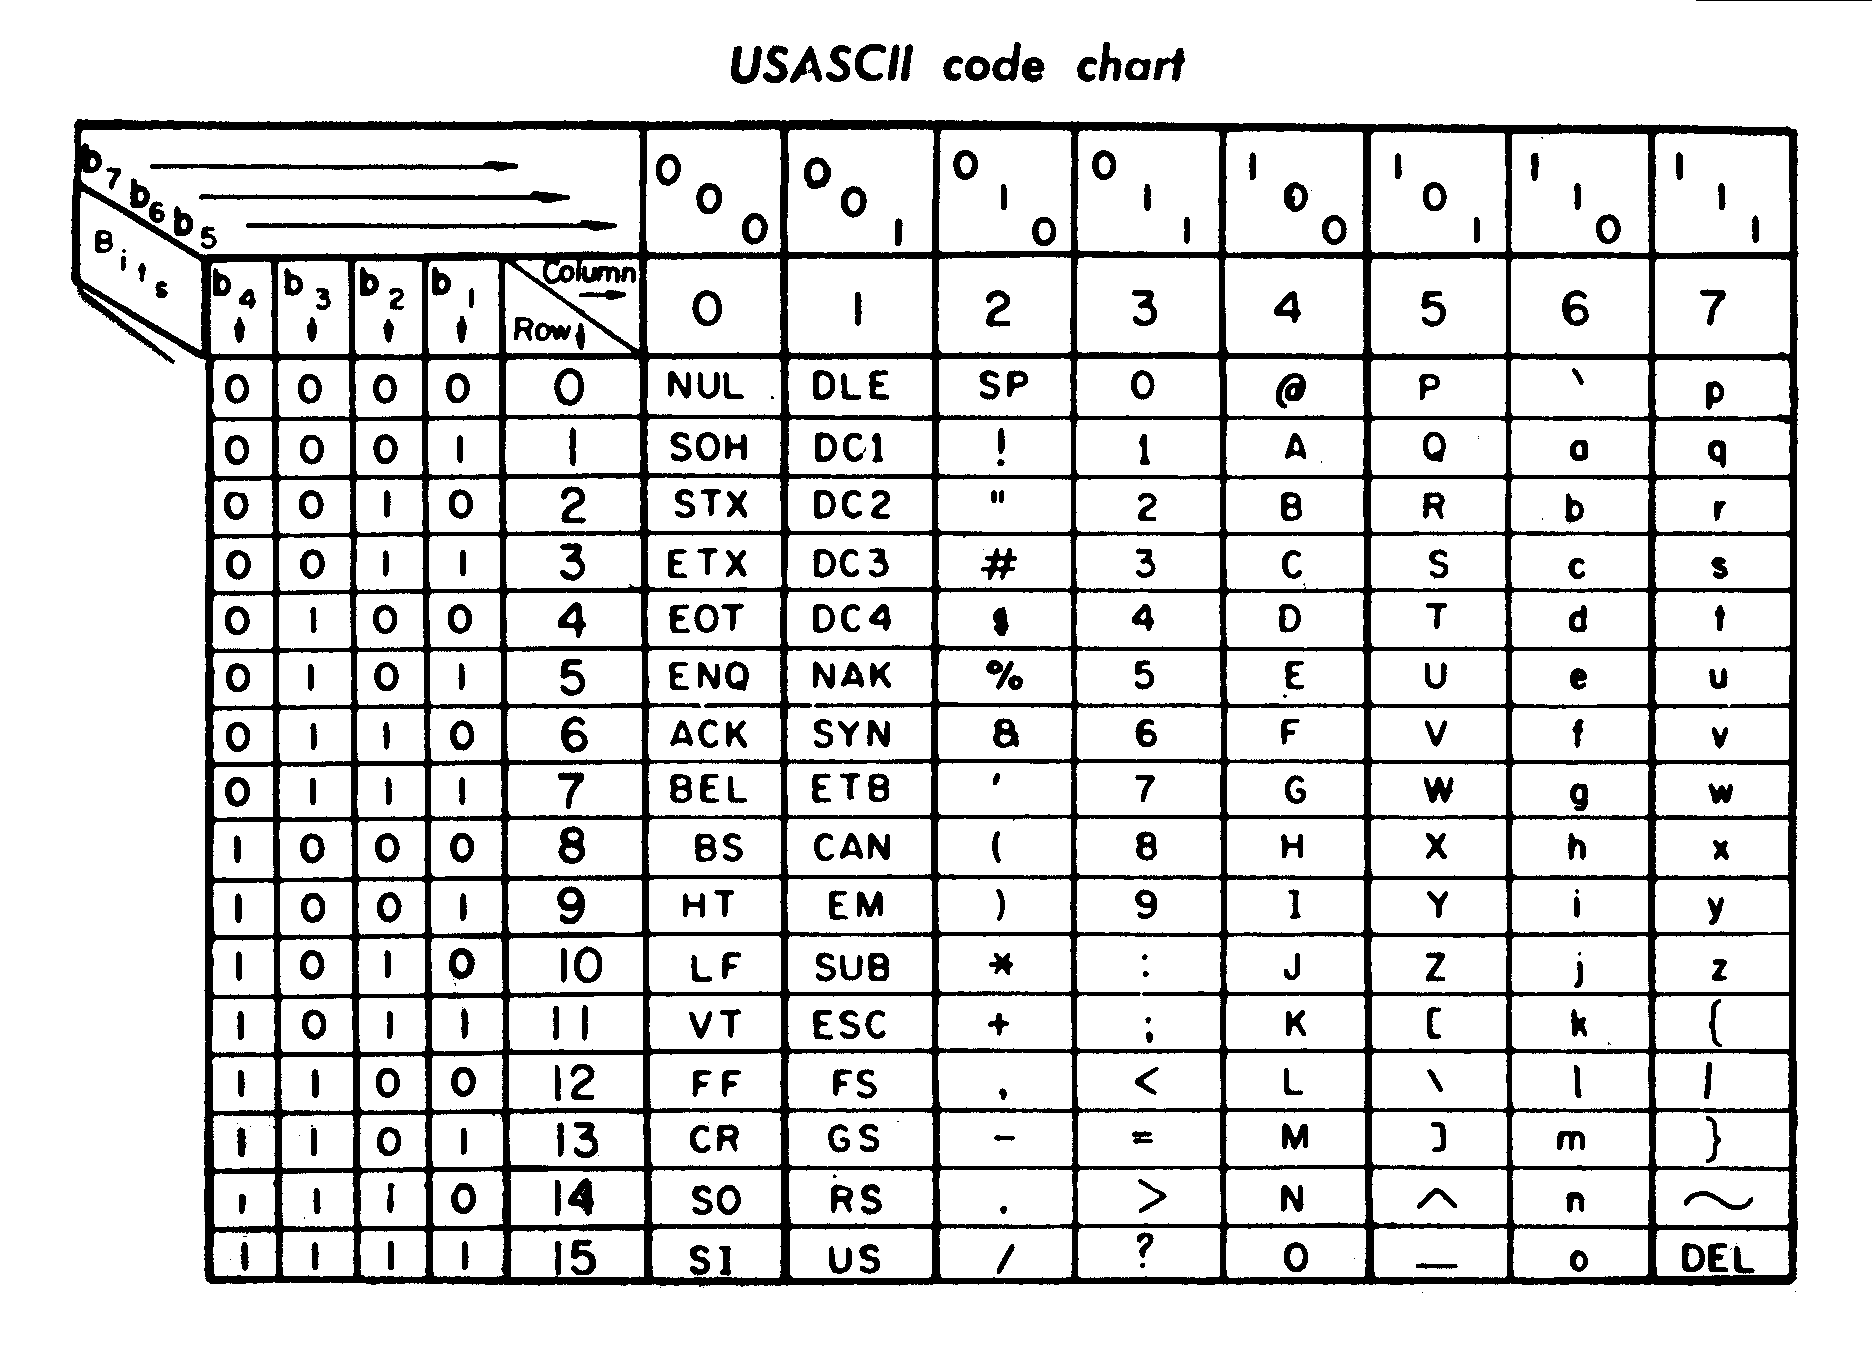
\includegraphics{subtex/ascii-chart.png}

The problem arose when computer technology spread beyond the labs of Silicon
Valley and government offices of Washington. In other countries, there was a
need to encode a vast array of linguistic forms, including diacritical marks,
right-to-left scripts, and pictographic writing systems. In the 1990s, many
national encoding schemes were created to represent languages other than
English. Most of these were "extensions" of ASCII, meaning the original
128-character ASCII set remained intact, and non-English characters were added
to the higher integer values. The only problem here is that they were not
intercompatible, meaning that documents might not "play nice" when transferred
between countries or languages.

Unicode and its dominant encoding scheme UTF-8 intend to alleviate these
problems by collecting all of the world's glyphs into one system. The 127
characters in ASCII are represented using the same single-byte codes, which
means that no conversion for existing ASCII files is necessary, and these will
not become bloated in a new conversion scheme. But the encoding scheme takes
advantage of modern computer's greater storage capacities to represent 1,112,064
distinct characters. 
